\chapter{Message Propagation}
\label{chp:message_propagation}

Um eine hohe Flexibilität, unabhängige Entwicklung und eine bessere Verteilung der Last zu erreichen, ist die Unabhängigkeit zwischen der Siemens GNA Software und dem Backend von großer Bedeutung.
Durch die Aufteilung des Systems in kleine Teile entsteht ein verteiltes System in der Service-Oriented Architecture. Jedoch ist die Koordination und die Synchronisation solcher Systeme äußerst komplex und verlangt hohen Aufwand. Mit dieser Problematik befasst sich die \emph{Message Propagation} und bietet eine Reihe an Lösungsansätze, um diese Komplexität zu vereinfachen. In dieser Arbeit ist sich für die Technologie der Messaging-Systeme entschieden worden, die es verschiedenen Teilen eines verteilten Systems ermöglicht, unabhängig voneinander zu kommunizieren. Dadurch kann die entwickelte Applikation eine starke Entkopplung, Skalierbarkeit und eine schnelle Echtzeitverarbeitung gewährleisten.

Im nächsten Abschnitt werden die verteilten Systeme der Service-Oriented Architecture mit Fokus auf der internen Kommunikation erklärt. Die darauf folgenden Kapitel werden die Eigenschaften und Struktur von Enterprise Messaging Systemen vertieft erläutern. Des Weiteren werden zwei populäre Implementierungen dieser Technologie, nämlich RabbitMQ und Apache Kafka, vorgestellt.

\section{Verteilte Systeme in der Service-Oriented Architecture}

In der \emph{Service-Oriented Architecture} (SOA) werden Softwareressourcen als Services verpackt, die eigenständige Module darstellen. Diese bieten standardisierte Geschäftsfunktionalitäten und sind unabhängig vom Zustand oder Kontext anderer Dienste. Es wird eine Sammlung von Services erstellt, die miteinander kommunizieren können, indem eine API verwendet wird, um Nachrichten von einem Service an ein anderes zu übermitteln oder eine Aktivität zwischen zwei oder mehreren Teilen des Systems zu koordinieren. In der Abbildung \ref{fig:serviceOrientatedArchitecture} ist ein einfacher Aufbau mit den Abhängigkeiten der einzelnen Module eines SOAs zu erkennen. Auf diese Weise kann mit SOA ein sehr flexibles, entkoppeltes System geschaffen werden. Jedoch ist die Koordination der Services eine große Herausforderung. Dadurch sind einige Kommunikationstechniken entstanden, welche später im Kapitel \ref{kommunikationstechnikenInVerteilteSysteme} beschrieben werden. Des Weiteren weisen verteilte Systeme gewisse Eigenschaften und Merkmale auf, mithilfe denen eine Bewertung des Systems durchgeführt werden kann. Diese werden nun im Kapitel \ref{eigenschaftenVonVerteiltenSystemen} erläutert.
\cite{papazoglouServiceOrientedArchitectures2007}

\begin{figure}
    \centering
    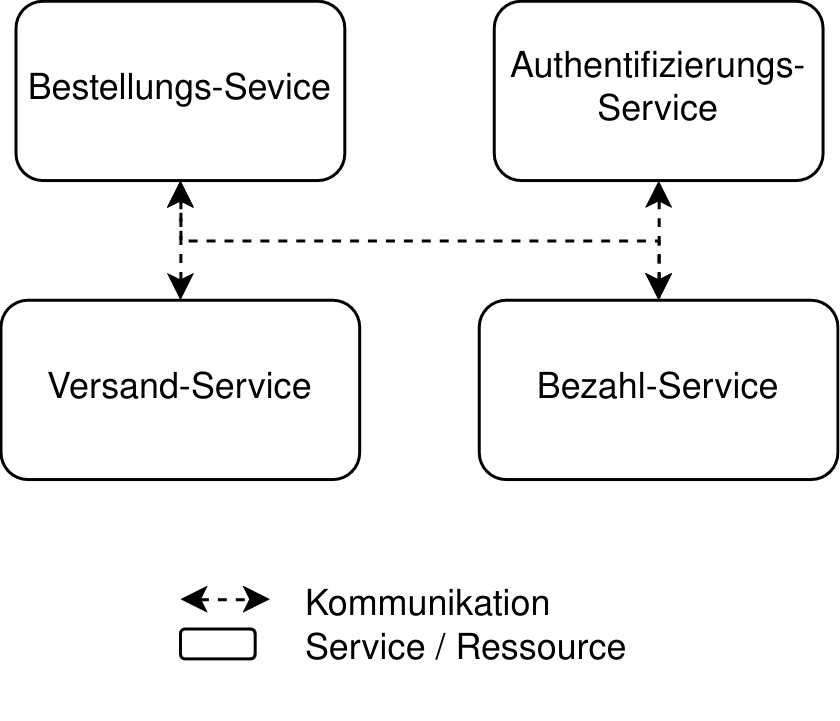
\includegraphics[width=0.6\textwidth]{content/img/Research/Message_Services/serviceOrientatedArchitecture.png}
    \caption{Darstellung eines Systems, welches auf einer Service-Oriented Architecture beruht}
    \label{fig:serviceOrientatedArchitecture}
\end{figure}
\FloatBarrier

\subsection{Eigenschaften zur Bewertung von verteilten Systeme}
\label{eigenschaftenVonVerteiltenSystemen}
Die Entwicklung eines verteilten Systems ist kein leichtes Unterfangen. Dadurch ist es sehr wichtig, die Funktionsfähigkeit des Anwendungssystems ermitteln zu können. In der folgenden Liste sind die Eigenschaften und Merkmale eines SOA-Systems aufgezählt, welche eine leichte Bewertung ermöglichen. \cite{toshevLearningRabbitMQBuild2016,curryMessageOrientedMiddleware2004}

\begin{itemize}
	\item \textbf{Kopplung}: Eine hohe Entkopplung der einzelnen Komponenten spielt eine wichtige Rolle, um eine unabhängige Entwicklung und eine hohe Flexibilität der Anwendung zu erreichen.
	\item \textbf{Latenz}: Da in verteilten Systemen die Ressourcen aufgeteilt werden, ist es von Bedeutung, die Kommunikation der Komponenten mit einer niedrigen Verzögerung zu gewährleisten.
	\item \textbf{Skalierbarkeit}: Moderne Anwendungen müssen in der Lage sein, sich an die Belastung anzupassen, die durch die Interaktion der Benutzer mit der Software entsteht. Dies ermöglicht einen reibungslosen, nicht frustrierenden Ablauf für die Benutzer.
	\item \textbf{Wartbarkeit}: Verteilte Systeme müssen in der Lage sein, ihre Komplexität zu abstrahieren und dadurch eine leichte Wartbarkeit zu realisieren. Denn nicht überschaubare Systeme stellen langfristig einen erheblichen Kostenfaktor in der Entwicklung und Wartung dar.
	\item \textbf{Zuverlässigkeit}: Um eine erfolgreiche Anwendung zu gewährleisten, bedarf es einer Software mit hoher Robustheit und Zuverlässigkeit, da Fehler in der Anwendung unerwünschte Auswirkungen haben können, die in Produktivsystemen nicht toleriert werden können.
	\item \textbf{Verfügbarkeit}: Wenn es zu Ausfällen von Anwendungssystemen kommt, können erhebliche Kosten in Millionenhöhe entstehen. Daher ist es von entscheidender Relevanz, diese Ausfälle zu minimieren und eine stetige Verfügbarkeit zu gewährleisten.
	\item \textbf{Erweiterbarkeit}: Im Lebenszyklus einer Anwendung ist die kontinuierliche Erweiterbarkeit tief verankert, da sich Geschäftsszenarien ständig ändern können. Eine Software, die die Fähigkeit besitzt, sich flexibel an diese Anforderungen anzupassen, bietet erhebliche Vorteile.
\end{itemize}

\subsection{Kommunikationstechniken in verteilte Systeme}
\label{kommunikationstechnikenInVerteilteSysteme}

Die Koordination und Kommunikation in verteilten Systemen können schnell zu einer äußerst anspruchsvollen Aufgabe werden, sobald das System eine bestimmte Größe erreicht. Die Synchronisation und Koordination von Services im Allgemeinen bei solchen Systemen ist nicht trivial. Beispielsweise müssen Sie sich nur einmal vorstellen, aus wie vielen kleinen Services alle Google Apps bestehen müssen, damit Millionen von Nutzern gleichzeitig damit arbeiten können. Es ist offensichtlich, dass solche Systeme leicht zu einem unüberschaubaren Netzwerk von Abhängigkeiten werden können. Ein weiterer Punkt, welcher zu beachten ist, wäre: Was passiert, wenn ein Service ausfällt und damit der Zugriff auf eine Ressource nicht mehr möglich ist? Eine Ausnahmesituation dieser Art kann leicht zu Inkonsistenzen im System führen oder im Extremfall eine Kettenreaktion auslösen, die zu einem totalen Ausfall der gesamten Anwendung führt. Damit solche Szenarien vermieden werden können und der Informationsaustausch der Module des verteilten Systems verlässlich und einfach gestaltet werden kann, haben sich verschiedene Kommunikationstechniken etabliert, welche in den nachfolgenden Unterkapiteln erklärt und verglichen werden. \cite{google2009services}

\subsubsection{Direkte Kommunikation zwischen den Services}

Die trivialste Lösung wäre eine Form von \emph{Remote Procedure Calls (RPC)} zwischen den einzelnen Teilen des verteilten Systems. Ein RPC ist eine Technik, die es einem Programm ermöglicht, eine Funktion oder Methode in einem anderen entfernten Programm aufzurufen, als ob sie lokal aufgerufen würde. Allerdings führt dies zu einer hohen Kopplung, da die einzelnen Services direkt miteinander kommunizieren, wie es in der Darstellung \ref{fig:direkteKommunikationMOM} zu erkennen ist. 
Die Natur dieser Kommunikationstechnik benötigt eine synchrone Übertragung, weil die Kommunikationspartner stets auf die Rückmeldung des anderen warten müssen, um Gewissheit zu erlangen, dass die Nachricht erfolgreich übermittelt wurde. Die synchrone Übertragung hat eine geringere Skalierbarkeit im Gegensatz zur asynchronen Übertragung, da durch das Warten auf die Rückmeldung Verzögerungen entstehen.    
Wenn diese Systeme eine gewisse Größe erreichen, werden sie zu undurchsichtigen Netzen an Abhängigkeiten, was zu aufwendiger Wartung und erschwerter Erweiterung des Systems führt. Dennoch können die Anforderungen an die Echtzeitkommunikation erfüllt werden, da alle Services direkt miteinander kommunizieren.
\cite{toshevLearningRabbitMQBuild2016,curryMessageOrientedMiddleware2004}

\begin{figure}
    \centering
    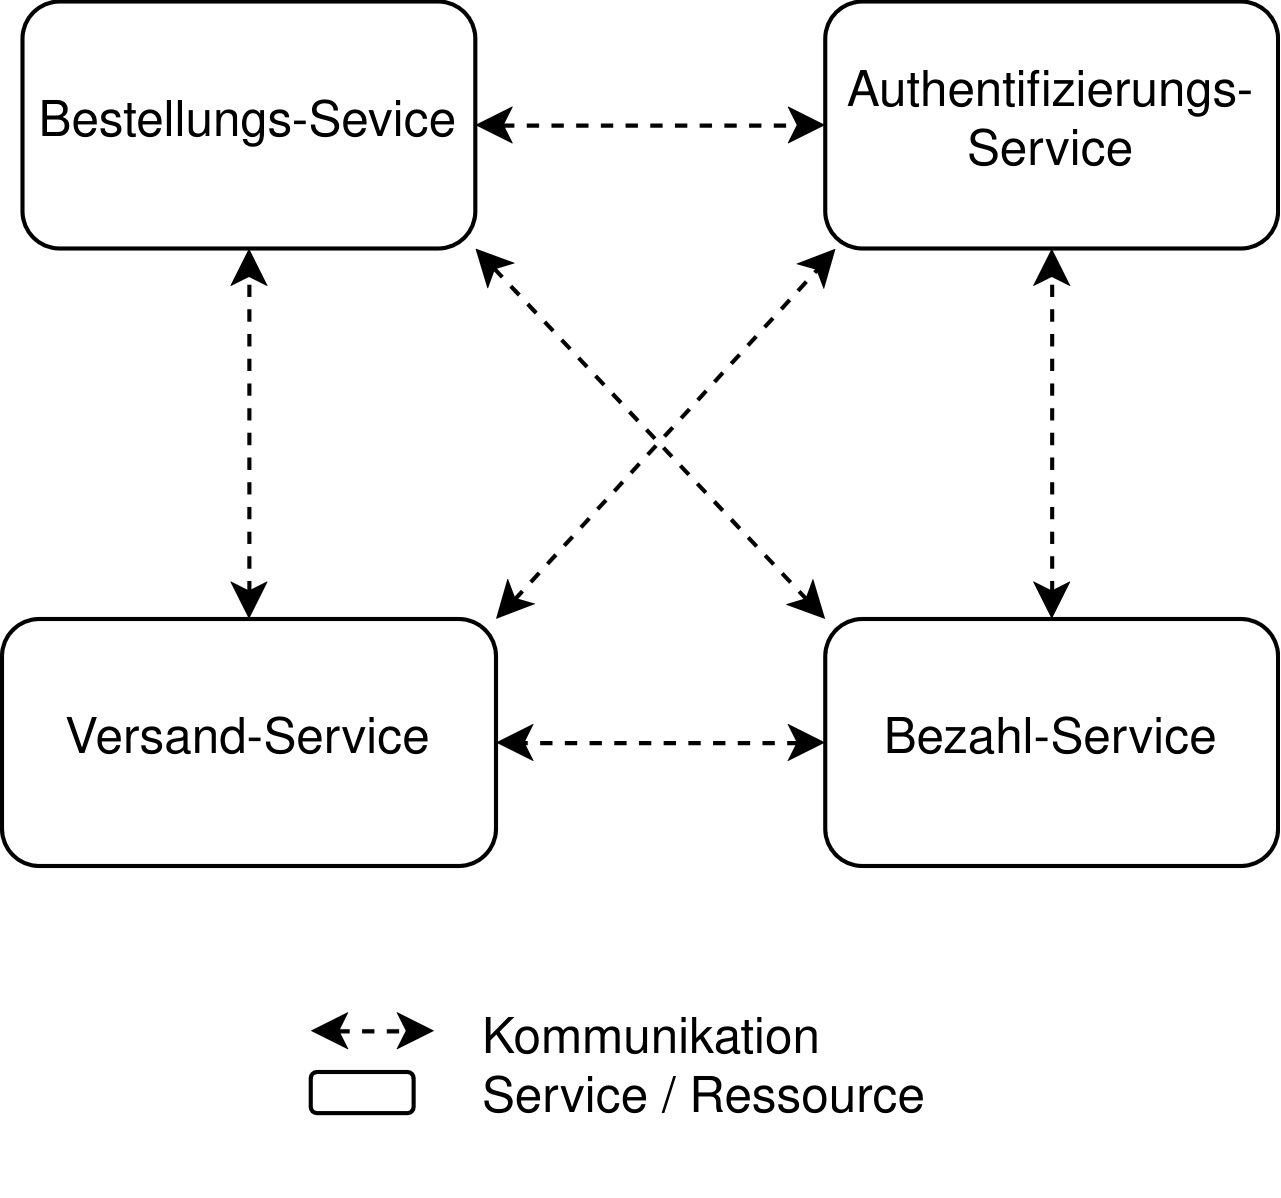
\includegraphics[width=0.6\textwidth]{content/img/Research/Message_Services/direktKommunikationMOM.png}
    \caption{Ein Beispiel für ein verteiltes System mit direkter Kommunikation \cite{curryMessageOrientedMiddleware2004}}
    \label{fig:direkteKommunikationMOM}
\end{figure}
\FloatBarrier

\subsubsection{Verwendung einer gemeinsamen Datenbank}

Eine weitere Möglichkeit des Informationsaustauschs könnte die Kommunikation über eine gemeinsame Datenbank sein. In dieser Architektur sind alle Services von dem gleichen Datenbank-Schema abhängig, welches die Koppelung reduziert. Durch die Zentralisierung der Kommunikationswege, wie es in der Abbildung \ref{fig:datenbankKommunikationRabbit} erkennbar ist, wird ein sehr übersichtlicher Aufbau des verteilten Systems geschaffen. Weitere Services können auch leicht integriert werden, da sie nur mit dem Datenbank-Schema kommunizieren müssen. Wenn jedoch das Datenbank-Schema angepasst wird, müssen alle Module angepasst werden. Dieser Prozess könnte mit großem Aufwand verbunden sein. Eine hohe Skalierbarkeit zu erreichen, ist in den meisten Fällen sehr herausfordernd, da jedes Modul den zentralen Punkt belastet, insbesondere bei relationalen Datenbanken, da diese von Natur aus schwer zu skalieren sind. \cite{toshevLearningRabbitMQBuild2016,curryMessageOrientedMiddleware2004}

\begin{figure}
    \centering
    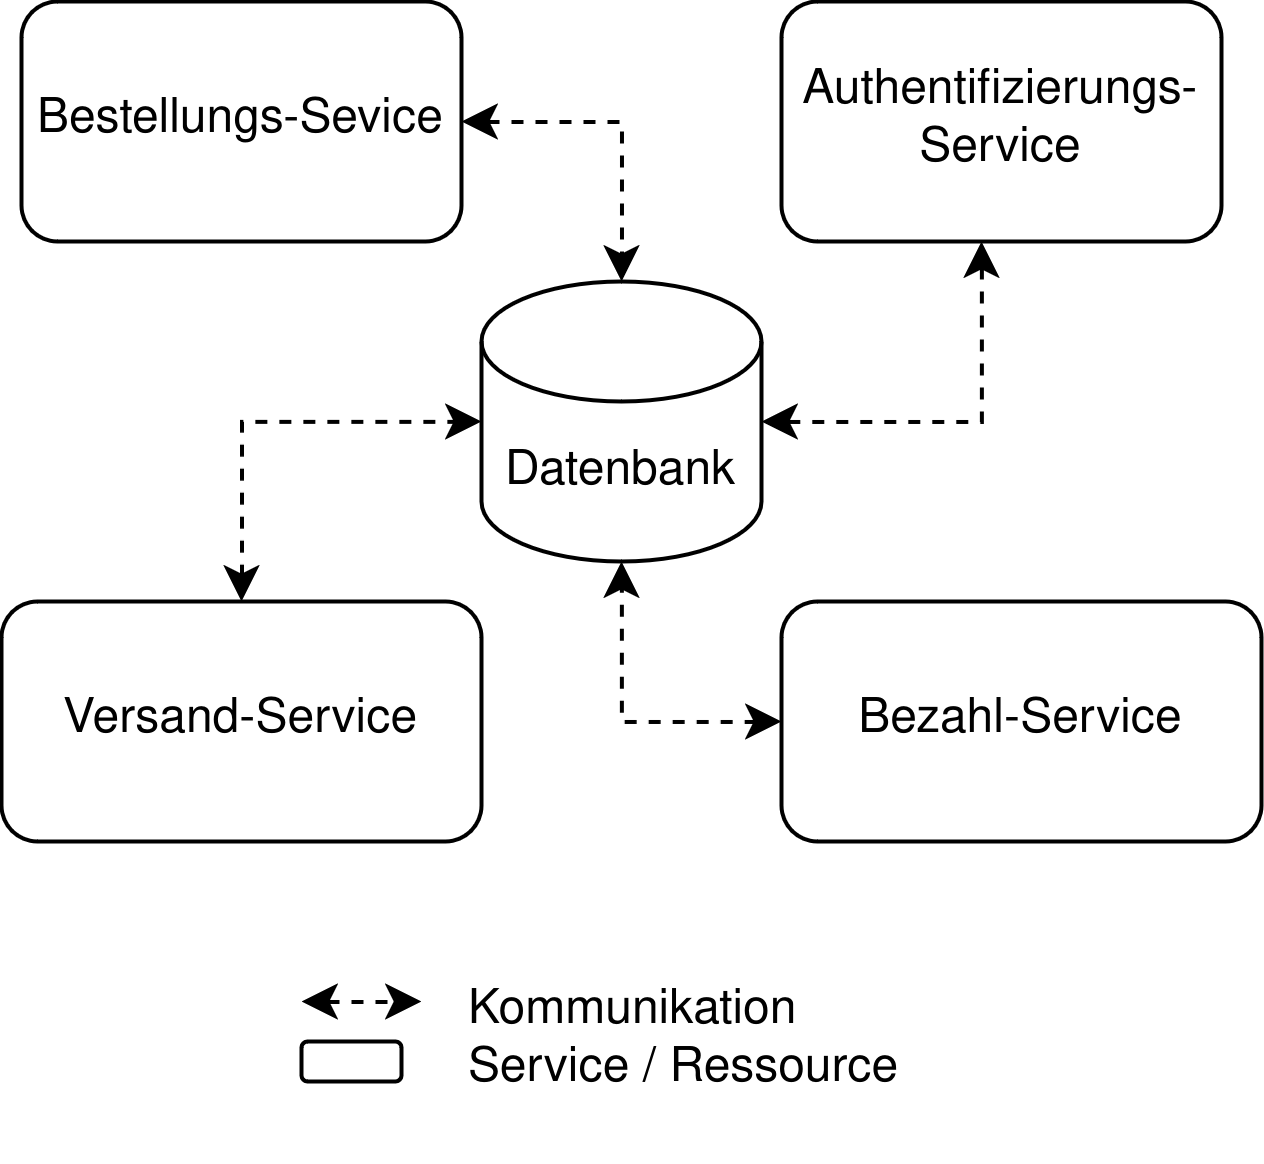
\includegraphics[width=0.6\textwidth]{content/img/Research/Message_Services/datenbankKommunikationRabbit.png}
    \caption{System mit Datenbank als zentraler Kommunikationskomponente}
    \label{fig:datenbankKommunikationRabbit}
\end{figure}
\FloatBarrier

\subsubsection{Nutzung von einem Messaging System}

Bei der Verwendung von einem oder mehreren Messaging Systemen wird jegliche Kommunikation über einen oder mehrere zentrale Punkte geleitet, wie in der Abbildung \ref{fig:messagingSystemsKommunikation} zu erkennen ist. Ein Sender schickt seine Nachricht zu dem Nachrichten-System, welches die Information an einen oder mehrere Empfängern weiterleitet. \cite{curryMessageOrientedMiddleware2004}

Durch den zentralisierten Aufbau bleibt das verteilte System übersichtlich und wartbar, was beim Auftreten eines Fehlers zu einer erheblich vereinfachten Ursprungssuche führt.
Die Kopplung der Services ist sehr niedrig, weil das Messaging-System eine zusätzliche Schicht zwischen dem Empfänger und dem Sender vertritt. Somit können auch beispielsweise alte Services leicht mit moderneren ersetzt werden. \cite{toshevLearningRabbitMQBuild2016}

Die Übertragung ist in diesem Fall vollständig asynchron, da die Kommunikationspartner nicht auf die Antwort des anderen warten müssen, weil die Nachricht einfach an einen Vermittler übergeben wird. Die Skalierbarkeit von verteilten Systemen, welche Messaging Systeme verwenden, ist aufgrund deren asynchronen Natur grundsätzlich sehr hoch und kann daher auch zu Spitzenzeiten die Last der Benutzer standhalten. \cite{toshevLearningRabbitMQBuild2016}

Zusätzlich wird auch die zuverlässige Nachrichtenübertragung sichergestellt. Dies rüht daher, weil Nachrichten, die nicht zugestellt werden können, da der Empfänger momentan nicht erreichbar ist, zwischengespeichert werden, damit diese zu einem späteren Zeitpunkt an den Empfänger gesendet werden können. \cite{curryMessageOrientedMiddleware2004}

Des Weiteren ermöglicht eine Architektur mit Messaging-Systemen eine einfache Erweiterbarkeit. Denn durch das Hinzufügen eines weiteren Services werden keine bestehenden Kommunikationskanäle beeinträchtigt. Somit kann das System mittels neuen Komponenten ohne großen Aufwand um dessen Funktionalität erweitert werden. Dies trägt dazu bei, dass das System flexibel bleibt und mit den Anforderungen des Unternehmens oder der Anwendung mitwachsen kann. \cite{curryMessageOrientedMiddleware2004}

In Bezug auf die Latenz bietet die Verwendung von Messaging-Systemen oft niedrige Verzögerungszeiten, insbesondere aufgrund der asynchronen Übertragung. Dies ermöglicht eine effiziente und zeitnahe Kommunikation zwischen den verschiedenen Komponenten eines verteilten Systems. \cite{curryMessageOrientedMiddleware2004}

\begin{figure}
    \centering
    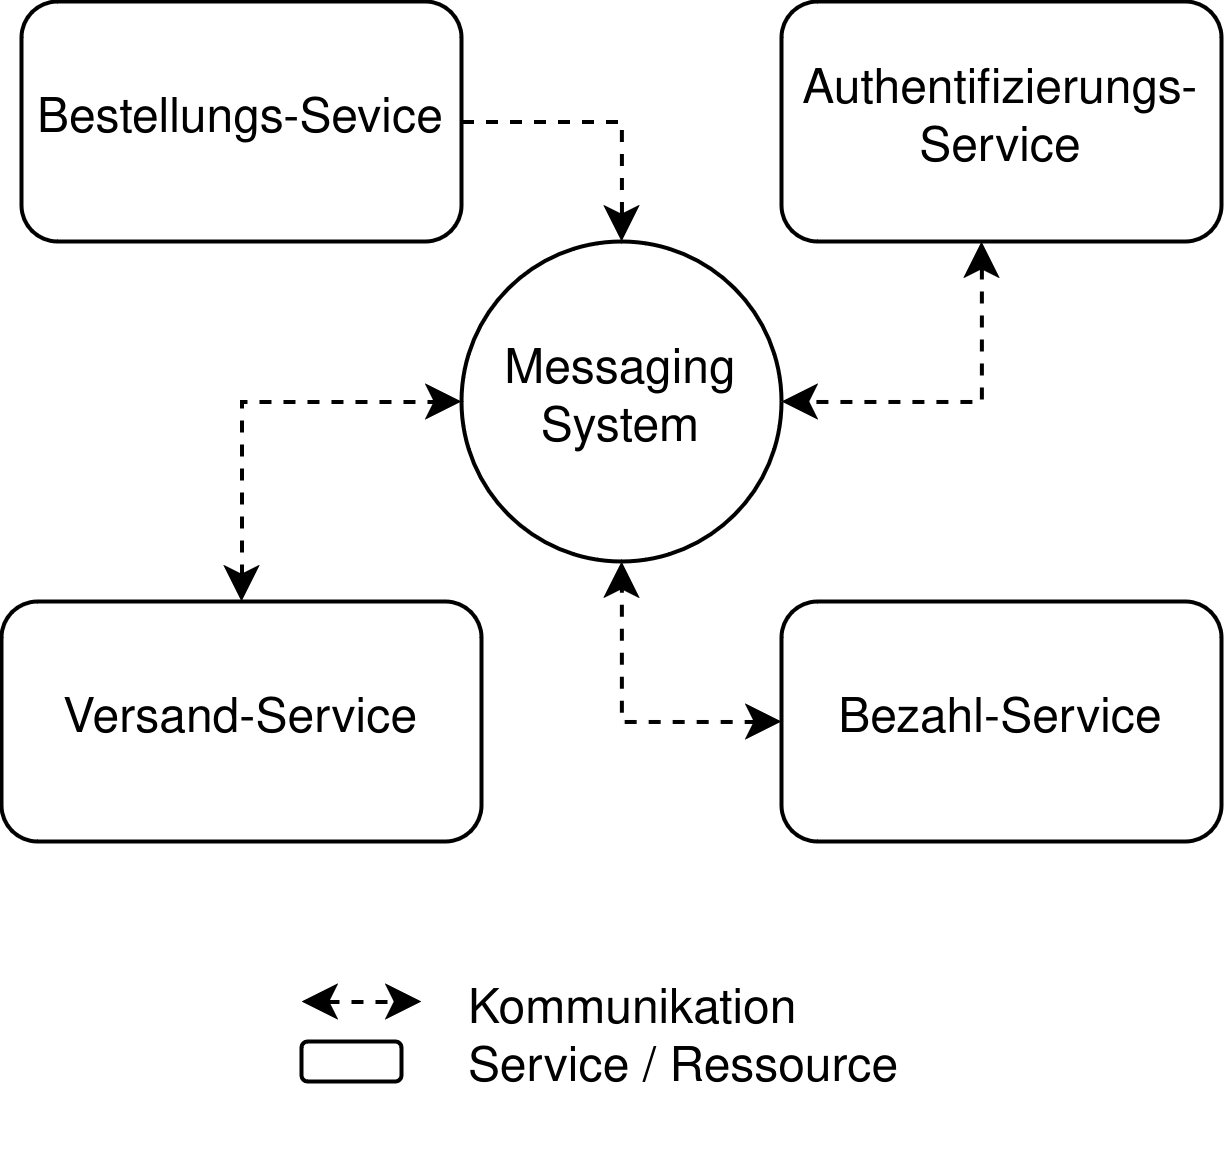
\includegraphics[width=0.6\textwidth]{content/img/Research/Message_Services/kommunikationWithMessagingSystemRabbitMQ.png}
    \caption{Messaging System als zentraler Kommunikationsknoten}
    \label{fig:messagingSystemsKommunikation}
\end{figure}
\FloatBarrier

Im folgenden Kapitel werden wir nun detailliert auf die Funktionsweise eines EMS eingehen.

\section{Enterprise Messaging Systems}

Messaging-Systeme bieten eine hervorragende Lösung für die Kommunikation in verteilten Systemen, wie es im Kapitel \ref{kommunikationstechnikenInVerteilteSysteme} dargelegt ist. In diesem Kapitel wird auf den Aufbau und die Funktionsweise von solchen Nachrichten-Systemen eingegangen. \cite{curryMessageOrientedMiddleware2004}

Durch ein Messaging System sind Sender (\emph{Publisher}) und Empfänger (\emph{Consumer}) stark entkoppelt, da sie über einen gemeinsamen Vermittler – dem Messaging-System – kommunizieren. Die Sender müssen Nachrichten an das Messaging System übertragen und die Empfänger erhalten die Nachrichten vom Nachrichten-System. \cite{curryMessageOrientedMiddleware2004}

Damit die Nachrichten nicht durcheinander geraten, wird pro Anwendungsfall ein Kommunikationskanal (\emph{Queue}) definiert, über welchen sich die Kommunikationspartner austauschen können. Wie viele Sender oder Empfänger es in einem Kanal gibt, ist völlig beliebig. Beispielsweise könnte es in einem Monitoringsystem mehrere Sensoren geben, welche als Publisher ihre gemessenen Daten einem Kanal übertragen. Auf der anderen Seite könnte es einen Consumer geben, welcher die Daten in eine Datenbank schreibt und einen zweiten, welcher die Daten für die Auswertung entgegennimmt. In der Abbildung \ref{fig:beispeilSensorenMessagingSysteme} ist dieses Beispiel visualisiert. \cite{curryMessageOrientedMiddleware2004}

Zusätzlich kann das Messaging System Nachrichten validieren, speichern, transformieren und durch vordefinierte Regeln an die geeigneten Empfänger weiterleiten (\emph{Routen}). Dadurch wird ein einheitlicher und zuverlässiger Weg für die Kommunikation ermöglicht. \cite{curryMessageOrientedMiddleware2004}

\begin{figure}
    \centering
    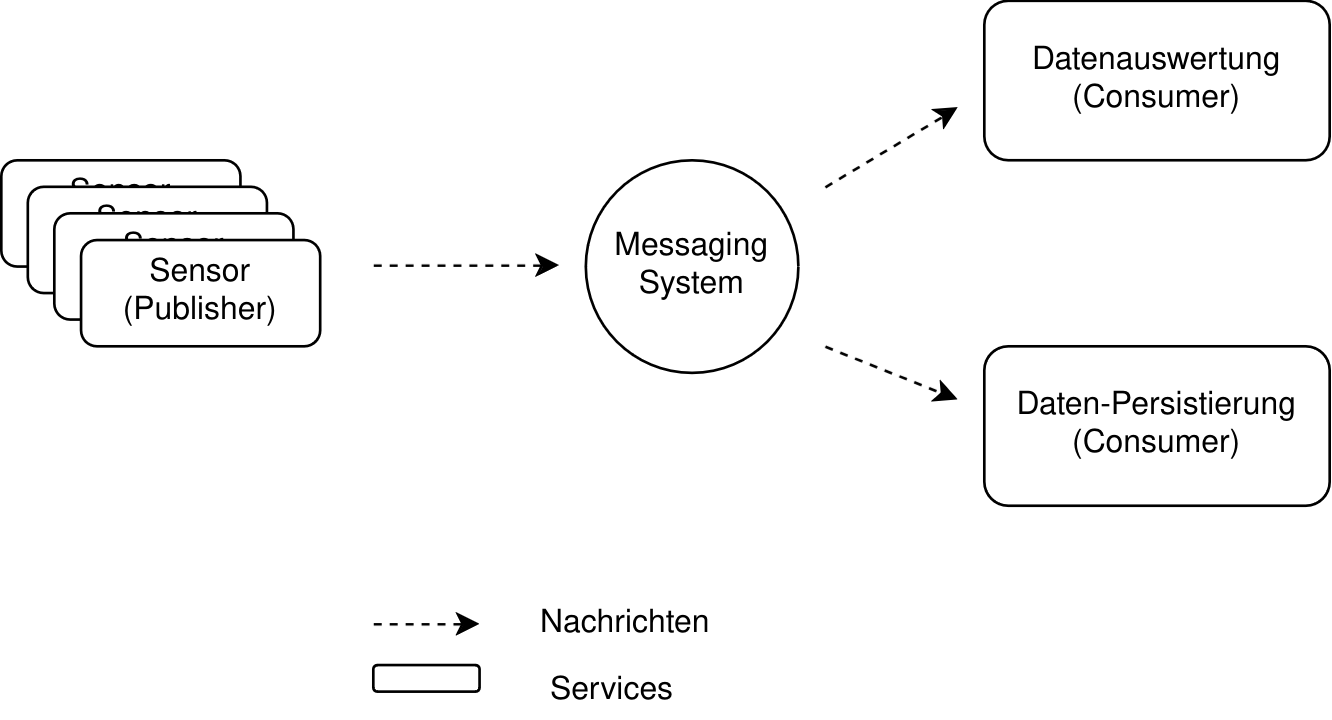
\includegraphics[width=0.6\textwidth]{content/img/Research/Message_Services/beispeilSensorenMessagingSysteme.png}
    \caption{Ein Beispiel für ein verteiltes System mit ein zentrales Messaging System}
    \label{fig:beispeilSensorenMessagingSysteme}
\end{figure}
\FloatBarrier

\subsection{Enterprise Service Bus}

Organisationen stehen oft vor der Herausforderung, verschiedene Technologien und Protokolle in das verteilte System integrieren zu müssen, um eine effektive Kommunikation und Interaktion zwischen ihren Systemen zu ermöglichen. In diesem Kontext spielen Messaging-Systeme eine entscheidende Rolle, da sie als Bindeglied zwischen den verschiedenen Komponenten dienen und den reibungslosen Austausch von Informationen unterstützen. \cite{menge2007enterprise}

Die Verwendung verschiedener Protokolle wie REST, SOAP, JMX, AMQP oder RPC in einem verteilten System kann zu einer hohen Komplexität führen. Insbesondere wenn es darum geht, diese Protokolle miteinander zu verknüpfen. Hier kommt der \emph{Enterprise Service Bus (ESB)} ins Spiel. Ein ESB fungiert als zentrale Kompatibilitätsschicht, die es ermöglicht, verschiedene Systeme und Protokolle nahtlos miteinander zu verbinden. \cite{menge2007enterprise}

Diese Integration kann durch verschiedener Adapter realisiert werden, die Protokolle auf andere konvertieren. Dadurch kann der ESB die Interoperabilität zwischen Systemen erleichtern. Dies ermöglicht eine effiziente Integration von bestehenden Systemen sowie die Anbindung von Systemen, die an bestimmte Protokolle gebunden sind. Trotz seiner Vorteile erfordert die Implementierung und Wartung eines ESB jedoch einen erheblichen Aufwand, um den unterschiedlichen Kommunikationsanforderungen der Protokolle gerecht zu werden. In der Abbildung \ref{fig:enterpriseMessagingBus} ist ein einfaches Anwendungsbeispiel eines ESBs dargestellt. \cite{toshevLearningRabbitMQBuild2016,menge2007enterprise}

\begin{figure}
    \centering
    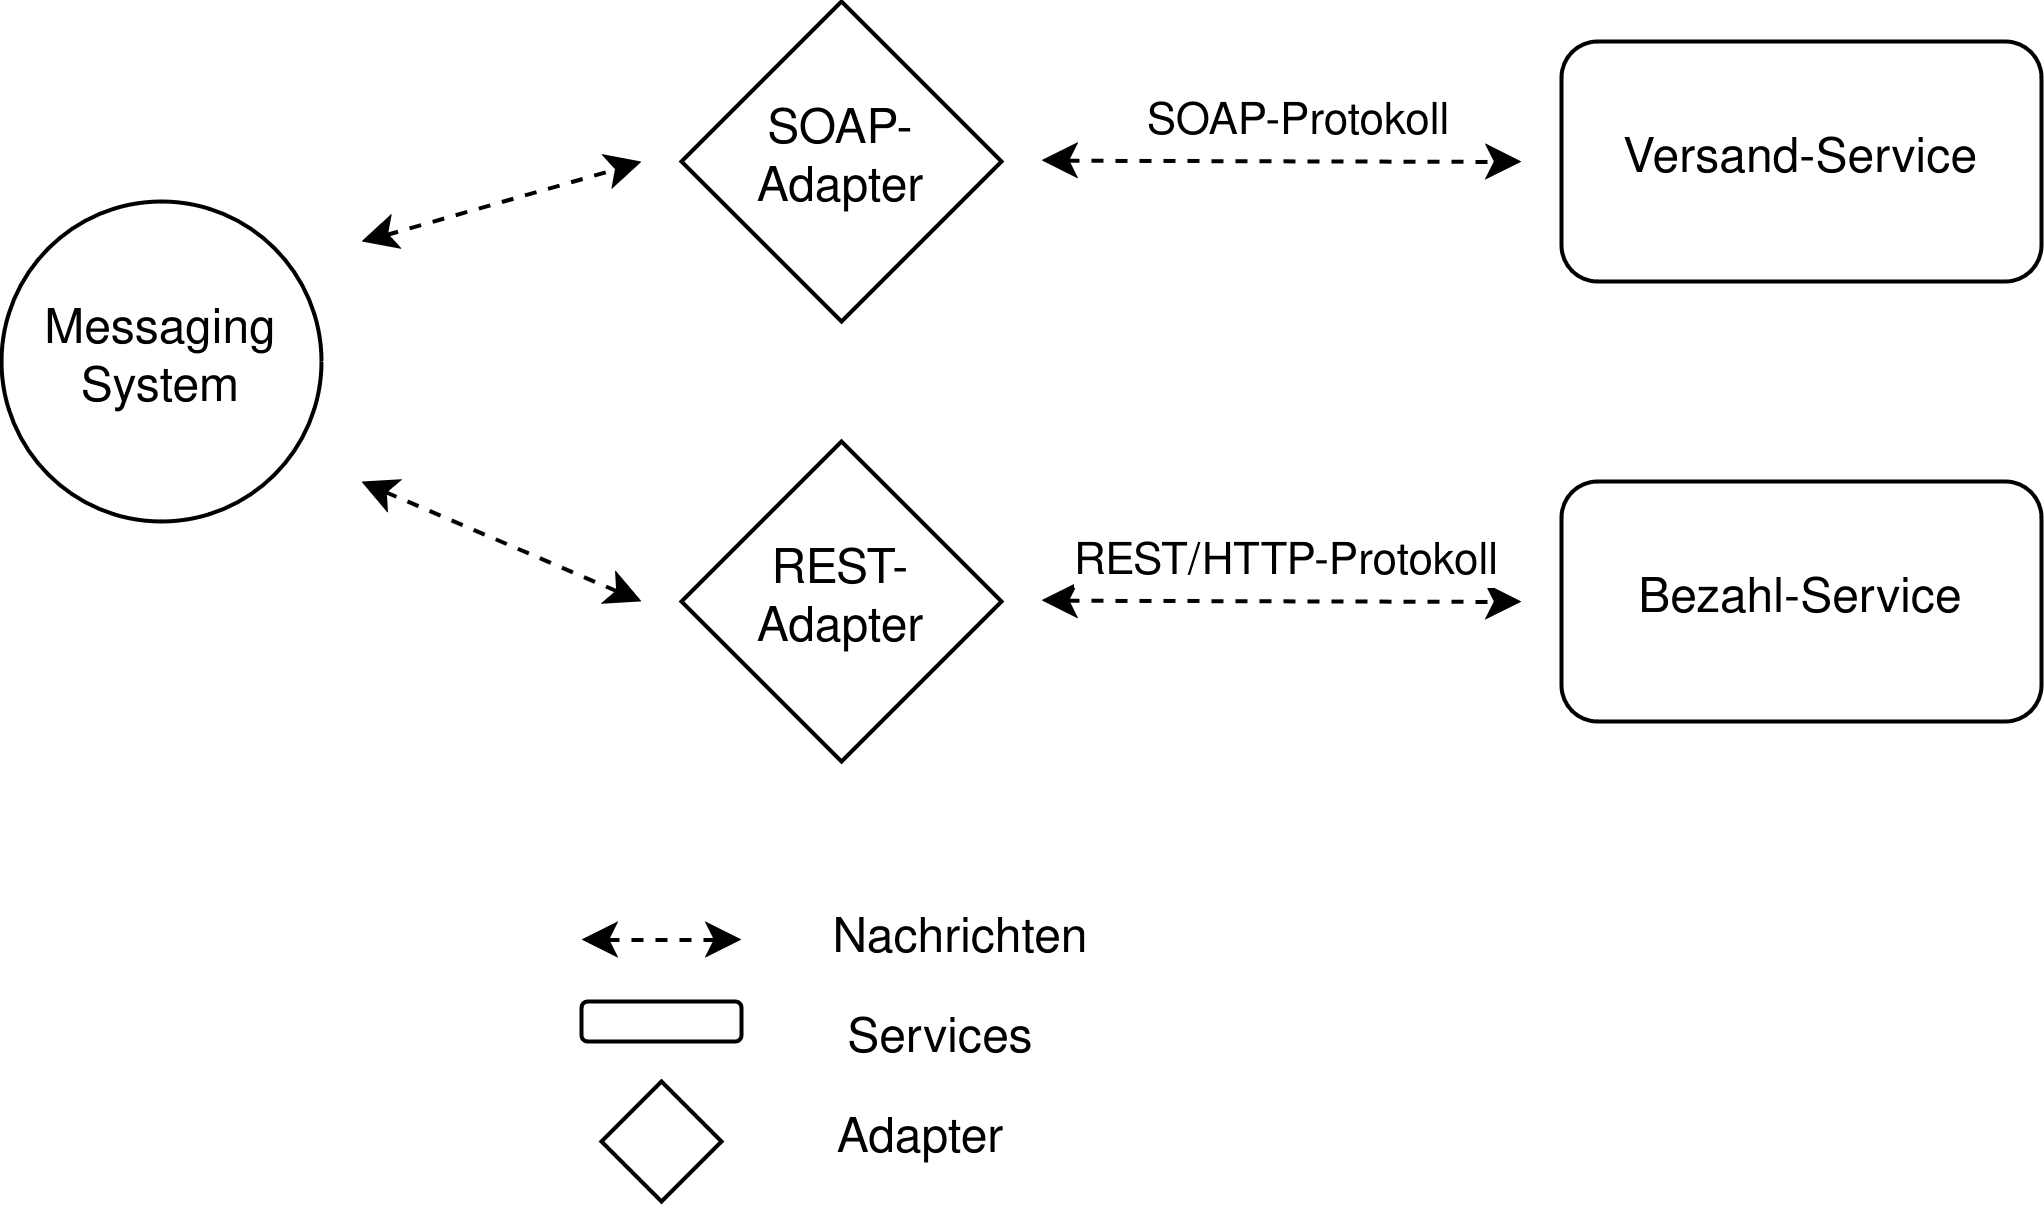
\includegraphics[width=0.6\textwidth]{content/img/Research/Message_Services/esb.png}
    \caption{Ein einfacher Enterprise Service Bus}
    \label{fig:enterpriseMessagingBus}
\end{figure}
\FloatBarrier

\subsection{Nachrichten}

Das Konzept der Nachricht bildet das Herzstück der Kommunikation innerhalb eines Messaging-Systems. Eine Nachricht besteht in der Regel aus verschiedenen Bestandteilen, die ihre Struktur und Funktionalität definieren. Typischerweise umfasst eine Nachricht die folgenden Elemente: \cite{toshevLearningRabbitMQBuild2016}

\begin{itemize}
	\item \textbf{Header} -- Der \emph{Header} einer Nachricht enthält wichtige Metadaten, die für die Verarbeitung und Weiterleitung der Nachricht entscheidend sind. Dazu gehören Informationen wie das Encoding der Nachricht, Routing-Informationen zur Bestimmung des Zielorts der Nachricht und möglicherweise auch sicherheitsrelevante Daten, die für die Authentifizierung und Autorisierung relevant sind.

	\item \textbf{Body} -- Der \emph{Body} einer Nachricht enthält die eigentlichen Daten, die übermittelt werden sollen. Dies können beispielsweise Textnachrichten, strukturierte Daten im JSON- oder XML-Format, Binärdaten oder Daten in anderen Formaten sein. Dies kommt ganz auf die Anforderungen und den Zweck der Nachricht an. Jedoch sollte vermerkt werden, dass die Menge der Daten im Body gering gehalten werden sollte, damit verhindert wird, dass das Messaging System überladen wird. Wenn Daten von mehreren Gigabyte verschickt werden müssen, wäre die Übertragung eines Links für den Zugriff auf ein externes Speichersystem, wo die Daten sich befinden, die optimale Lösung.
\end{itemize}

Die Kombination aus Header und Body ermöglicht es, Informationen effizient und strukturiert innerhalb des Messaging-Systems zu transportieren. Dadurch wird eine zuverlässige und effiziente Kommunikation innerhalb des Messaging-Systems gewährleistet.

\subsection{Queues}

Die \emph{Message Queue} ist ein essenzieller Teil des Messaging-Systems. Sie bieten die Funktionalität, Nachrichten für einen bestimmten Anwendungsfall im Messaging System zu speichern. Die Sender reihen Nachrichten in die Queue ein und die Empfänger nehmen die Nachrichten über die Queue entgegen, wie es in der Darstellung \ref{fig:messagingQueueMOM} zu erkennen ist. \cite{curryMessageOrientedMiddleware2004}

Die standardmäßigen Queues folgen dem \emph{First-In, First-Out (FIFO)} Prinzip. Das bedeutet, dass diejenigen Nachrichten zuerst bearbeitet werden, welche als Erstes in die Queue eingefügt worden sind. Dies gewährleistet eine vorhersehbare Abwicklung der Nachrichten, wodurch eine ordnungsgemäße Kommunikation zwischen den verschiedenen Komponenten des Systems ermöglicht wird. \cite{curryMessageOrientedMiddleware2004}

Die Sender und Empfänger können dabei völlig unabhängig voneinander mit der Queue interagieren. Dies bedeutet, dass Sender Nachrichten in die Queue senden können, ohne sich um die Verfügbarkeit der Empfänger kümmern zu müssen. Gleichzeitig können Empfänger Nachrichten aus der Queue abrufen und verarbeiten, ohne auf direkte Interaktion mit den Sendern angewiesen zu sein. \cite{curryMessageOrientedMiddleware2004}

\begin{figure}
    \centering
    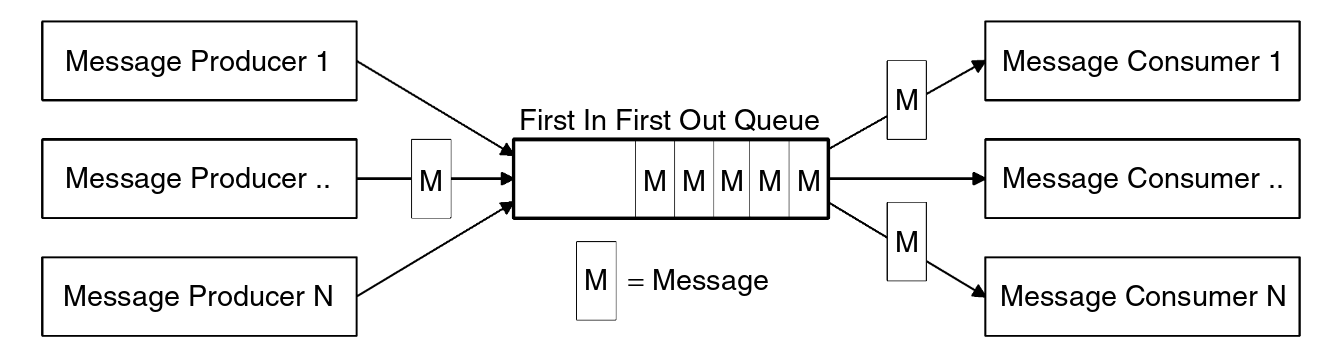
\includegraphics[width=0.8\textwidth]{content/img/Research/Message_Services/messagingQueueMOM.png}
    \caption{Eine Queue  \cite{curryMessageOrientedMiddleware2004}}
    \label{fig:messagingQueueMOM}
\end{figure}
\FloatBarrier

Es können viele Parameter von einer Queue konfiguriert werden, hierzu zählen unter anderen:

\begin{itemize}
	\item Der Name der Queue
	\item Die Größe der Queue
	\item Der Sortieralgorithmus für die Nachrichten
	% \item Der Schwellenwert für die Sicherung von Nachrichten
\end{itemize}

Eine spezielle Art der Queue sind die \emph{Dead-Message Queues}, sie beinhalten Nachrichten, welche nicht zugestellt werden konnten. 
Typischerweise beinhalten diese Queues Nachrichten, die im Body kein gültiges Format oder eine ungültige Ziel-Queue haben. Der Zweck einer Dead-Message Queue besteht darin, Nachrichten aufzubewahren, die nicht erfolgreich verarbeitet werden konnten, damit sie später untersucht und möglicherweise erneut bearbeitet werden können. 
Durch die Verwendung einer Dead-Message Queue können Messaging-Systeme eine bessere Fehlerbehandlung und -toleranz bieten, da sie es ermöglicht, fehlgeschlagene Nachrichten zu isolieren und separat zu behandeln.
\cite{curryMessageOrientedMiddleware2004}

\subsection{Message Broker und Cluster}

Die Kernkomponente eines Messaging Systems ist der \emph{Message Broker}, dieser erhält die Nachrichten der Services und leitet sie anschließen zu den Ziel-Services weiter. Der Broker übernimmt unter anderen folgende Aufgaben: \cite{narkhedeKafkaDefinitiveGuide2017}

\begin{itemize}
	\item \textbf{Erhalt der Nachrichten} – Der Broker empfängt eingehende Nachrichten von den Services und sorgt für das zuverlässige Senden an die Ziel-Services.
	\item \textbf{Speichern der Nachrichten} – Der Broker kann Nachrichten vorübergehend speichern, um sicherzustellen, dass sie nicht verloren gehen, falls ein Ziel-Service vorübergehend nicht verfügbar ist.
	\item \textbf{Routing von Nachrichten} – Der Broker leitet eingehende Nachrichten an die entsprechenden Ziel-Services weiter, basierend auf definierten Routing-Regeln oder -Kriterien.
\end{itemize}

Um Ausfallsicherheit und Skalierbarkeit zu gewährleisten, können Messaging Systems in \emph{Clustern} betrieben werden, die aus mehreren Message-Brokern bestehen. Diese Cluster ermöglichen die Replikation und Verteilung von Nachrichten über mehrere Broker hinweg. Es gibt zwei gängige Architekturen für Messaging-Cluster: \cite{narkhedeKafkaDefinitiveGuide2017}

\begin{itemize}
	\item \textbf{Master-Slave} – In dieser Architektur sind die Broker in \emph{Master} und \emph{Slave} unterteilt. Der Master-Broker übernimmt die Hauptaufgaben der Nachrichtenverarbeitung und -verteilung, während die Slave-Broker als Backup dienen und im Falle eines Ausfalls des Masters einspringen können.
	\item \textbf{Peer-to-Peer} – Hier haben alle Broker im Cluster denselben Status und jede Nachricht wird in mehreren Brokern repliziert und gespeichert. Dadurch wird eine höhere Redundanz und Ausfallsicherheit erreicht, da jede Nachricht mehrere Kopien in verschiedenen Brokern hat.
\end{itemize}


\subsection{Kommunikationmodelle}

Ein Messaging System verendet eines oder mehrere Kommunikationsmodelle, welche die Grundlage für die Kommunikation der zu verbindenden Systeme definiert. \cite{curryMessageOrientedMiddleware2004}

\subsubsection{Point-to-Point}

In einem \emph{Point-to-Point} Kommunikationsmodell gibt es nur einen Sender und einen Empfänger pro Nachricht. Im Fall, dass es mehrere potenzielle Empfänger für eine bestimmte Nachricht gibt, kann nur ein einziger sie tatsächlich erhalten. In diesem Szenario werden die Empfänger manchmal als \emph{Competing-Consumers} bezeichnet, da sie um den Empfang der Nachricht konkurrieren. Dieses Modell ist in der Abbildung \ref{fig:point-to-pointMOM} dargestellt. \cite{curryMessageOrientedMiddleware2004}

Dieses Modell bietet einige nützliche Anwendungsfälle. Zum Beispiel kann es für eine einfache Form des \emph{Load Balancings} verwendet werden, indem die Nachrichten auf mehrere potenzielle Empfänger aufgeteilt werden. Auf diese Weise können Arbeitslasten gleichmäßig auf mehrere Systeme oder Prozesse verteilt werden, um die Gesamtleistung und Effizienz zu verbessern. \cite{curryMessageOrientedMiddleware2004}

Ein Real-World Szenario könnte wie folgt aussehen: Die Prüfung auf Viren in Dateien sollte über das Messaging System auf mehrere Server verteilt werden. Dazu wird der Link zu der Datei von einem Producer in eine spezielle Queue geschickt. Eine Gruppe von Scan-Servern steht bereit, um die eingehenden Links zu den Dateien zu empfangen und sie auf Viren zu überprüfen. Der Broker wird diese Nachricht einem dieser Server weiterleiten und somit den Scan-Vorgang starten.

\begin{figure}
    \centering
    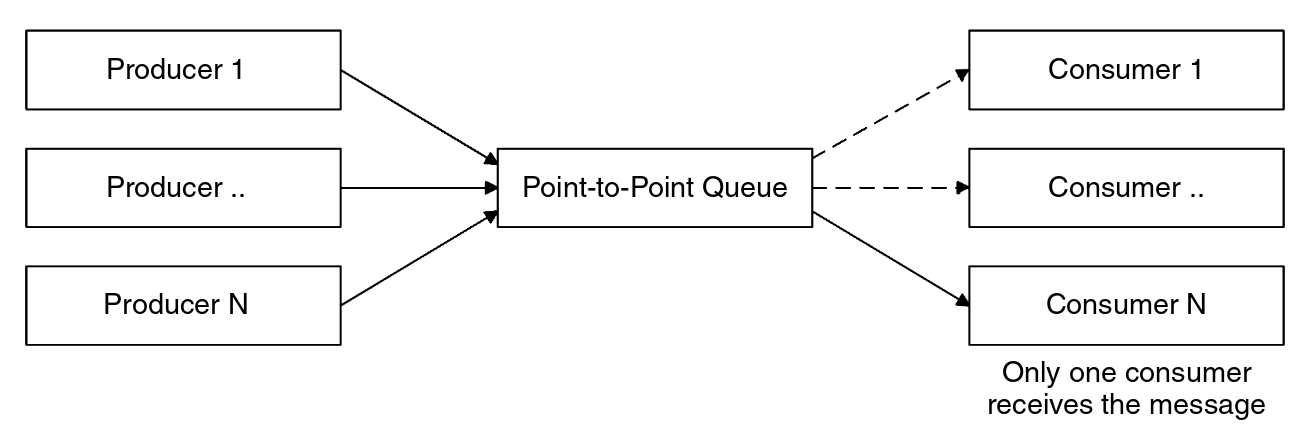
\includegraphics[width=0.8\textwidth]{content/img/Research/Message_Services/point-to-pointMOM.png}
    \caption{Das Point-to-Point Messaging Model \cite{curryMessageOrientedMiddleware2004}}
    \label{fig:point-to-pointMOM}
\end{figure}
\FloatBarrier

\subsubsection{Publish-Subscribe}

Im \emph{Publish-Subscribe Modell} werden Nachrichten mittels Nachrichten-Thema (\emph{Topics}) gruppiert. Beispielsweise könnten Sie für jeden Anwendungsfall ein Topic erstellen. Services, welche Nachrichten zu einem bestimmten Thema erhalten möchten, melden sich für den Erhalt der Nachrichten an (\emph{subscribe}). Wenn Sender die zu übertragende Information an Topics senden (\emph{publish}), werden immer alle Subscriber des Themas die Nachricht erhalten. Dieses Verhalten kann auch in der Abbildung \ref{fig:publish-subscribeMOM} erkannt werden. 
Außerdem gibt es keine Einschränkungen hinsichtlich der Rollen, die ein Service einnehmen kann. Ein Service kann sowohl Subscriber und Publisher sein. \cite{curryMessageOrientedMiddleware2004}

Ein anschauliches Beispiel wäre ein Benutzeraktivitäten-Tracking-System, welches aus einem Publisher und zwei Subscribern besteht. Der Producer, welcher die Aktivität des Benutzers sammelt,  verschickt die Informationen zu einem bestimmten Topic. Die zwei Empfänger des Topics verarbeiten diese Nachrichten, wobei der eine die Aktivitäten in eine Datenbank speichert und der andere diese für ein Empfehlungssystem auswertet. \cite{curryMessageOrientedMiddleware2004}

\begin{figure}
    \centering
    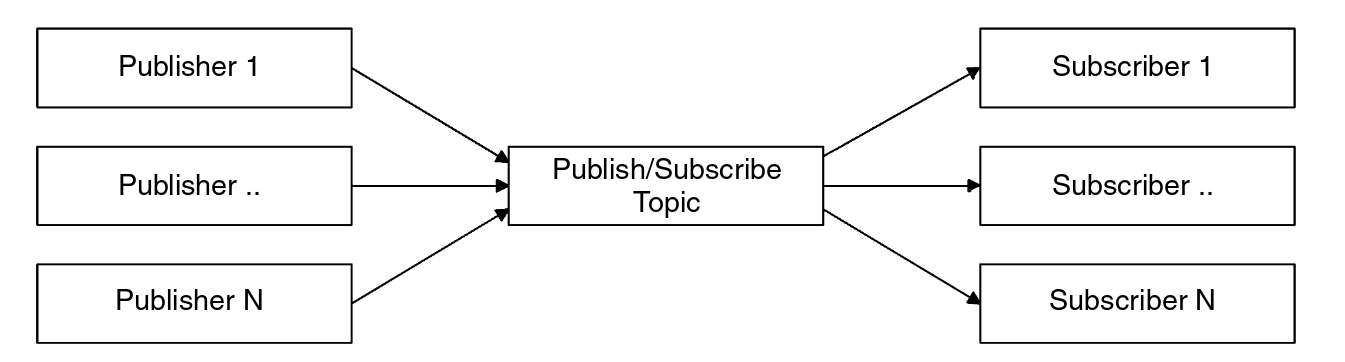
\includegraphics[width=0.8\textwidth]{content/img/Research/Message_Services/publish-subscribeMOM.png}
    \caption{Das Publish-Subscribe Messaging Model  \cite{curryMessageOrientedMiddleware2004}}
    \label{fig:publish-subscribeMOM}
\end{figure}
\FloatBarrier

\subsection{Konsummodus}

Dieser Aspekt der Kommunikation trifft nur auf die Empfänger zu und beschreibt, wie die Empfänger die Daten erhalten. Im Wesentlichen gibt es in diesem Zusammenhang zwei verschiedene Verbrauchsmodi, welche in dem folgenden Kapitel erklärt werden. Die Wahl des richtigen Modus ist entsprechend den Anforderungen, die das verteilte System erfüllen sollte, zu treffen.

\subsubsection{Push}

In \emph{Push-Modus} verteilt das Messaging System selber die Nachrichten an die Empfänger. Das heißt immer, wenn eine neue Nachricht beim Broker ankommt, wird diese direkt an den Empfängern weitergeleitet. Dieser Modus hat eine sehr hohe Echtzeit-Performance, da die zu übertragende Information ohne Verzögerung an die Empfänger weitergeleitet wird.

In diesem Modus besteht das Problem, dass der Message-Broker nicht über die Information verfügt, ob der Empfänger überhaupt in der Lage ist, weitere Nachrichten anzunehmen. Der Empfänger könnte überlastet werden, wenn in kurzer Zeit sehr viele Nachrichten übertragen werden, weil der Empfänger selbst nicht steuern kann, wie viele Nachrichten ihm zugeschickt werden. Um diese Problematik zu lösen, benötigen Sie einen \emph{Flow-Control} Mechanismus, damit die Übertragungsrate geregelt werden kann.  
\cite{curryMessageOrientedMiddleware2004,fuFairComparisonMessage2021}

\subsubsection{Pull}

Im \emph{Pull-Modus} muss der Nachrichtenempfänger immer beim Messaging System nach neuen Nachrichten fragen. Auf diese Weise kann der Empfänger die Verarbeitung von Nachrichten in Übereinstimmung mit seiner eigenen Kapazität steuern. Jedoch muss der Empfänger in einem geeigneten Zeitintervall diese Abfragen durchführen, um eine hohe Latenz zu vermeiden. Wenn dieses Intervall zu niedrig gewählt worden ist, werden die Message Broker durch diese vielen Anfragen jedoch selbst sehr stark belastet. Darüber hinaus ermöglichen diese Abfragen die Implementierung einer unkomplizierten Form von Lastenausgleich (Load Balancing), da jeder Empfänger eine Nachricht nur dann entgegennimmt, wenn er über die entsprechende Kapazität verfügt. \cite{curryMessageOrientedMiddleware2004,fuFairComparisonMessage2021}

\subsection{Quality-of-Service Garantien}

Damit die Operation eines verteilten Systems zuverlässig funktioniert, muss ein Messaging System bestimmte Garantien zusichern. Jedoch haben gewisse Garantien einen negativen Effekt auf die Performance des Systems. Beispielsweise wird für die Ordnung der Nachrichten in einem Cluster-System viel Rechenleistung benötigt. 
\cite{fuFairComparisonMessage2021}

\subsubsection{Zustellungsgarantien}

Um eine zuverlässige Übertragung zwischen Consumer und Producer zu gewährleisten, sind verschiedene Strategien für die Nachrichtenübertragung verfügbar: \cite{fuFairComparisonMessage2021}

\begin{itemize}
	\item \textbf{At-Most-Once} – Hier wird eine Nachricht höchstens einmal übertragen. Es besteht jedoch die Möglichkeit, dass die Nachricht während des Übertragungsvorgangs verloren geht.
	\item \textbf{At-Least-Once} –  Diese Methode stellt sicher, dass eine Nachricht mindestens einmal vollständig übertragen wird. Es kann jedoch vorkommen, dass eine Nachricht mehrmals übertragen wird, um sicherzustellen, dass sie erfolgreich empfangen wurde.
	\item \textbf{Exactly-Once} – Bei dieser Strategie wird garantiert, dass jede Nachricht genau einmal übertragen wird. Dadurch wird sichergestellt, dass Duplikate vermieden werden und keine Nachrichten verloren gehen.
\end{itemize}

Die meisten Messaging-Systeme bieten die At-Most-Once oder At-Least-Once Garantie. Die Exactly-Once wird durch ihre Komplexität nur von manchen Message-Systemen angeboten. \cite{fuFairComparisonMessage2021}

Eine weitere Garantie, welche durch Messaging Systems erreicht werden kann, ist die \emph{disk-based Retention}, also die Speicherung der Nachrichten auf der Festplatte. Dies bringt einen großen Vorteil mit sich, weil Nachrichten über einen längeren Zeitraum im Messaging System aufbewahrt werden können. Da die Messages auf der Festplatte persistiert werden und sich nicht nur im RAM befinden, kann kein Datenverlust auftreten. Es kann zum Beispiel während Wartungsarbeiten an den Empfängern trotzdem sichergestellt werden, dass keine Nachrichten verloren gehen. \cite{narkhedeKafkaDefinitiveGuide2017}

\subsubsection{Sortierungsgarantien}

Ein weiter wichtige Aspekt ist die Reihenfolge der Nachrichten, jedoch hat diese Garantie nur bei Cluster-Systemen Relevanz. Denn in einem Cluster ist die Synchronisierung der Ordnung über mehrere Broker hinweg sehr ressourcenintensiv. Die folgenden Strategien für die Nachrichtenordnung sind in der Praxis üblich: \cite{fuFairComparisonMessage2021}

\begin{itemize}
	\item \textbf{No-Ordering} – Bei dieser Strategie gibt es keine festgelegte Sortierung für die Nachrichten. Dies ermöglicht eine maximale Performance, da keine Ressourcen für die Synchronisierung der Nachrichten verwendet werden.
	\item \textbf{Partition-Ordering} - Nachrichten werden innerhalb eines einzelnen Brokers geordnet, aber es gibt keine Garantie für die Sortierung über mehrere Broker hinweg. Diese Strategie bietet eine gewisse Ordnung, ohne die Performance übermäßig zu beeinträchtigen.
	\item \textbf{Global-Ordering} - Hier werden die Nachrichten über den gesamten Cluster hinweg geordnet. Dies bietet maximale Konsistenz, aber es geht auf die Kosten der Performance, da die Synchronisierung der Nachrichtensortierung zwischen den Brokern sehr aufwendig sein kann.
\end{itemize}

Wenn die Sortierungsgarantie \emph{Global-Ordering} aus Performancegründen nicht angewendet werden kann, ist es erforderlich, die Kommunikation der Services so zu gestalten, dass die Reihenfolge der Nachrichten keine Bedeutung hat. Jedoch kann diese Anforderung in der Umsetzung erhebliche Probleme verursachen. Die Synchronisierung von Aktionen und die Gewährleistung der Konsistenz der Daten können erschwert werden, da keine garantierte Reihenfolge der Nachrichten vorhanden ist. Dies erfordert eine sorgfältige Planung und Implementierung, um sicherzustellen, dass die Services trotz fehlender globaler Ordnung effizient und zuverlässig funktionieren. \cite{fuFairComparisonMessage2021}

\subsection{Protokoll für die Kommunikation mit dem Broker}

Das Protokoll zwischen dem Produer/Consumer und dem Message-Broker bildet die Grundlage des Informationsaustausches und hat eine sehr wichtige Bedeutung, da es die Funktionen des Messaging-Systemes definiert und eingrenzt. Die Kommunikationsstandards können in zwei Gruppen einteilt werden: in die open-source Protokolle und die closed-source Protokolle. Folgende weit verbreitete Protokolle werden zu den open-source Protokollen gezählt: \emph{AMQP}, \emph{XMPP}, \emph{REST} und \emph{STOMP}.  Die open-source Messaging-Protokolle sind den closed-source Protokollen in dem Aspekt Kopplung überlegen, da sie durch die offene Standardisierung die Abhängigkeit zu einem bestimmten Messaging System aufheben. Closed-source Protokolle sind oft Produkte von veränderten open-source Protokollen oder völlig neue geschaffene Kommunikationsdefinitionen, welche nur für bestimmte Systeme gedacht sind. \cite{fuFairComparisonMessage2021}

\subsection{Latenz und Durchsatz}

Der Begriff Latenz beschreibt die Zeit, die es benötigt, Nachrichten zwischen zwei Endpunkten über das Messaging System zu übertragen. Die folgenden Punkte haben den größten Einfluss auf diese Übertragungszeit: \cite{fuFairComparisonMessage2021}

\begin{itemize}
	\item Die Dauer für die Metadaten-Verarbeitung eines Pakets, wie zum Beispiel die Validierung oder das Routing.
	\item Die Zeit, welche für die Replikation eines Pakets in Anspruch genommen wird. Dieser Aspekt trifft insbesondere auf Messaging Systeme, welche in einer Cluster-Architektur arbeiten, zu.
	\item Die Speicherzugriffsverzögerung, welche durch die Methode und Ort des Zugriffs bestimmt ist. Zum Beispiel sind der Zugriffe auf RAM-gespeicherte Daten weniger zeitintensiv als Datenzugriffe auf eine Festplatte.
	\item Weitere Verzögerungen werden durch die Einhaltung der \emph{Quality-of-Service} Garantien erzwungen, wie beispielsweise die Ordnungsgarantien, welche einen besonders negativen Effekt haben.
\end{itemize}

\emph{Low Latency Messaging Services} minimieren diese Aspekte und können dadurch eine annähernde Echtzeitübertragung ermöglichen.

Der Durchsatz steht für die Menge an Daten, welche pro Zeiteinheit über das Messaging System übermittelt werden können. Damit die höchsten Durchsatzraten erreicht werden können, müssen die oben angeführten Punkte natürlich minimiert werden, aber es gibt noch einen weiteren Lösungsansatz: \emph{Batch-Processing}. 
In dieser Methode werden mehrere Nachrichten gesammelt und auf einmal übertragen, damit wird der Overhead erheblich reduziert. Jedoch ist diese Technik bekannt für den Kompromiss zwischen Durchsatz und Latenz. Denn um mehrere Nachrichten auf einmal übertragen zu können, muss gewartet werden, bis entsprechend viele Nachrichten angekommen sind. Deswegen können Sie bei manchen Messaging-Systemen, wie zum Beispiel Kafka \cite{narkhedeKafkaDefinitiveGuide2017}, je nach Anwendungsfall bestimmen, wie viele Nachrichten akkumuliert werden sollen. \cite{fuFairComparisonMessage2021}
\section{Vergleich von populären Enterprise Messaging Services}

Zwei der populärsten Messaging-Systeme, die in der Softwareentwicklung weit verbreitet sind, sind \emph{Apache Kafka} und \emph{RabbitMQ}. Beide Systeme bieten leistungsstarke Funktionen für das Messaging und adressieren unterschiedliche Anwendungsfälle und Anforderungen. In diesem Kapitel wird ein detaillierter Vergleich zwischen diesen Messaging-Systemen durchgeführt. Zusätzlich wird ihre Architektur, Funktionalitäten, Leistungsmerkmale, Einsatzszenarien und weitere relevante Aspekte analysiert, um Entwicklern und Architekten dabei zu helfen, die richtige Entscheidung für ihr Messaging-System zu treffen. Dabei werden sowohl die Stärken als auch die Schwächen dieser beiden Systeme beleuchtet, um einen umfassenden Einblick in ihre Unterschiede und Gemeinsamkeiten zu bieten.

\subsection{Apache Kafka}
\label{kakfaExplained}

Kafka ist ein hoch skalierbares und verteiltes Messaging System, welches bekannt für die Fähigkeit große Datendurchsatzraten erreichen zu können ist. Dieses System wird in der Scalar Programmiersprache geschrieben und hat eine sehr aktive Community, die das open-source Projekt ständig um Funktionen erweitert. Apache Kafka wird auch als Streaming-Plattform bezeichnet, da es die Anforderungen an Stream-Processing genügen kann. Stream-Processing ist die Datenverarbeitung an einen Fluss von Daten, also eine unendliche Serie an Daten. Das \emph{Messaging System} von Apache ist für diesen Anwendungsfall gut geeignet, da es in der Lage ist, die benötigten Durchsatzraten zu erreichen und eine Reihe an Stream-Processing Funktionalitäten besitzt, wie zum Beispiel \emph{Kafka Streams} oder \emph{KSQL}. Außerdem verfügt Apache Kafka über \emph{Connectors}, die zur Einbindung von externen Datenquellen oder Datensenken gedacht sind. Beispielsweise könnten Sie Daten über Kafka in einer Datenbank speichern oder über den \emph{MirrorMaker} zwei Kafka Cluster verbinden. \cite{narkhedeKafkaDefinitiveGuide2017,stopfordDesigningEventDrivenSystems2018}

Folgende Auflistung zählt die wichtigsten Vorteile von Apache Kafka auf: \cite{fuFairComparisonMessage2021}

\begin{itemize}
	\item \textbf{Hohe Skalierbarkeit} - Die Nachrichten werden in mehrere Partitionen aufgeteilt, die parallel beschrieben und ausgelesen werden können, was die Skalierbarkeit erhöht.
	\item \textbf{Hohe Verfügbarkeit} - Durch Replikation wird sichergestellt, dass Messages im Cluster redundant gespeichert werden, um Ausfallzeiten zu minimieren und die Verfügbarkeit zu maximieren.
	\item \textbf{Hohe Durchsatzraten} - Durch Batch-Verarbeitung werden große Mengen an Nachrichten gleichzeitig, effizient verarbeitet, was zu hohen Durchsatzraten führt.
	\item \textbf{Aufbewahrung der Nachrichten auf der Festplatte} - Die Nachrichten werden auf der Festplatte gespeichert, um Persistenz sicherzustellen und Datenverlust zu verhindern.
\end{itemize}

\subsubsection{Architektur von Kafka}

Grundsätzlich basiert die Architektur von Kafka auf das Messaging Model Publish-Subscribe. Die Nachrichten werden in verschiedene Topics unterteilt, und jedes Thema wird in mehreren Partitionen aufgeteilt. Diese Partitionen werden auf mehren Message Broker verteilt und repliziert, da Apache Kafka normalerweise als Cluster arbeitet. Partitionen werden benötigt, um die Nachrichten gleichmäßig auf die Message Broker aufzuteilen und den Empfängern das gleichzeitige Auslesen eines Themas zu ermöglichen. Wie es in der Abbildung \ref{fig:kafkaArchFairComparisonMessagingServices} zu sehen ist, verwendet Kafka die Peer-to-Peer-Replikationsmethode und Empfänger erhalten Nachrichten über den Konsummodus: \emph{Pull}. \cite{narkhedeKafkaDefinitiveGuide2017}

\begin{figure}
    \centering
    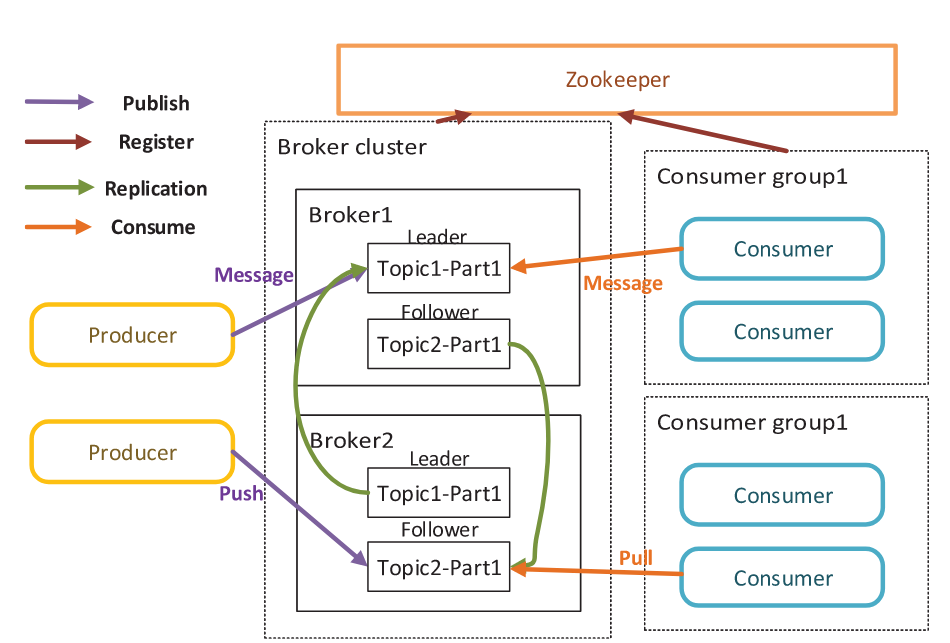
\includegraphics[width=0.8\textwidth]{content/img/Research/Message_Services/kafkaArchFairComparisonMessagingServices.png}
    \caption{Die Architektur des Apache Kafka Systems \cite{fuFairComparisonMessage2021}}
    \label{fig:kafkaArchFairComparisonMessagingServices}
\end{figure}
\FloatBarrier

Die Consumer können sich zu Gruppen zusammenschließen (\emph{Consumer-Group}) und können dadurch gemeinsam ein Topic verarbeiten. Consumer Groups können parallel mehrere Partitionen auslesen (siehe Abbildung \ref{fig:partitionsKafkaDefinitiveGuide}), jedoch werden die Messages auf die Empfänger aufgeteilt. Dadurch bieten sich Consumer-Groups perfekt für Anwendung bei \emph{Load Balancing} Use-Cases an. Außerdem benötigt Apache Kafka eine zusätzliche Applikation für das Verwalten und Koordinieren eines Clusters: \emph{Zookeeper}, zum Beispiel wird diese Applikation zur fehlerfreien und parallelen Auslesung von Topics benötigt.  \cite{narkhedeKafkaDefinitiveGuide2017}

\begin{figure}
    \centering
    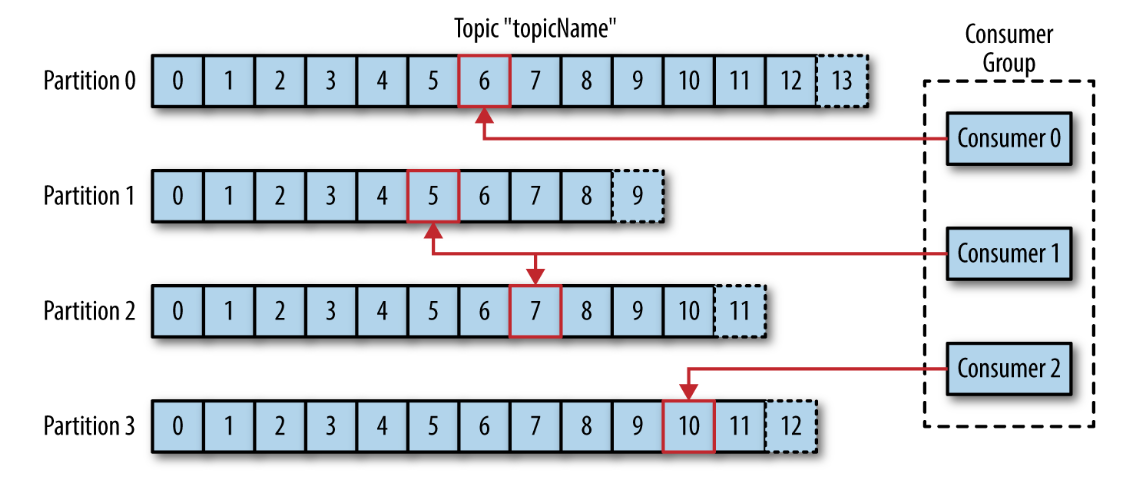
\includegraphics[width=0.8\textwidth]{content/img/Research/Message_Services/partitionsKafkaDefinitiveGuide.png}
    \caption{Eine Consumer-Group verarbeitet gemeinsam ein Topic. \cite{narkhedeKafkaDefinitiveGuide2017}}
    \label{fig:partitionsKafkaDefinitiveGuide}
\end{figure}
\FloatBarrier

Außerdem unterstützt Apache Kafka die Zustellungsgarantie At-Least-Once standardmäßig und die At-Most-Once Garantie kann bei Bedarf beim Producer eingestellt werden. Damit die Exactly-Once Zusicherung eingehalten werden kann, müssen aber Veränderungen am Ziel-Storage System bewerkstelligt werden. \cite{narkhedeKafkaDefinitiveGuide2017}

\newpage

Damit Kafka eine hohe Durchsatzrate erreicht werden kann, werden drei Methoden verwendet, die den \emph{Overhead} minimieren: \cite{narkhedeKafkaDefinitiveGuide2017}

\begin{itemize}
	\item \textbf{Die Nutzung von \emph{Zero-Copy}-Methoden}: Diese Technik wird verwendet, um Daten effizient zu übertragen, ohne dass Kopiervorgänge zwischen verschiedenen Pufferspeicherbereichen erforderlich sind. Im Kontext von Kafka wird diese Technik genutzt, um den Overhead bei der Datenübertragung zu minimieren und somit die Durchsatzraten zu verbessern.
	\item \textbf{Kafka überträgt Nachrichten in \emph{Batches}}: Durch die Stapelung von Nachrichten und deren gemeinsame Übertragung wird die Anzahl der Netzwerkverbindungen minimiert und die Effizienz der Datenübertragung gesteigert, was zu höheren Durchsatzraten führt.
	\item \textbf{Nachrichtenkomprimierung}: Diese Methode komprimiert Nachrichten, bevor sie über das Netzwerk übertragen werden, was die benötigte Netzwerkbandbreite reduziert und die Übertragungsgeschwindigkeit erhöht, was zu einer insgesamt verbesserten Durchsatzrate führt. Insbesondere wird die Leistung gesteigert, bei der Übermittlung von Nachrichten, welche gut komprimierbare Datenformate verwenden, wie zum Beispiel JSON.
\end{itemize}

Zusammenfassend lässt sich sagen, dass Apache Kafka optimal für Anwendungsfälle geeignet ist, welche eine hohe Skalierbarkeit und hohe Ausfallsicherheit benötigen. Des Weitern lässt sich Apache Kafka gut einsetzen in verteilte Systeme, welche die Anforderungen auf hohe Durchsatzraten bei der Übertragung von Nachrichten haben. Mit den Kafka Connectors ist es sogar möglich, die Anwendungsbereiche von einem Enterprise Service Bus zu decken. Jedoch ist bei der Verwendung von Kafka für Echtzeit-Kommunikation abzuraten, weil durch die Persistierung der Nachrichten auf der Festplatte Verzögerungen unvermeidbar sind. \cite{fuFairComparisonMessage2021}

\subsection{RabbitMQ}

RabbitMQ ist ein open-source Messaging Service, welcher um das Protokoll AMQP entwickelt wurde. Das System ist mit Erlang programmiert, da Erlang für das Entwickeln von verteilten Systemen geeignet ist, braucht es keine koordinierende Komponente wie Zookeeper. In der Abbildung \ref{fig:rabbitMQArchfairComparisonMessagingSystems} ist zu sehen, dass RabbitMQ auch als Cluster arbeiten kann, dafür werden die Queues auf mehrere Broker repliziert. Es gibt je Queue eine \emph{Master-Queue} und eine oder mehrere \emph{Backup-Queues}. Alle Operationen starten bei dem Master und werden zu den Backup-Queues weitergeleitet. Aber wenn die Master-Queue ausfällt, wird sofort eine Backup-Queue zur Master-Queue aufsteigen und somit ist eine hohe Ausfallsicherheit gegeben. Jedoch hat RabbitMQ kein gutes Design für Skalierbarkeit, weil die komplette Replikation der Queues nicht für hohe Auslastungen gut geeignet ist. \emph{Exchanges} sind für das \emph{Routen} der Nachrichten benötigt, sie können komplexe Routing-Anforderungen umsetzen, wie zum Beispiel die Verteilung der Nachrichten auf mehrere Queues. \cite{toshevLearningRabbitMQBuild2016}

\begin{figure}
    \centering
    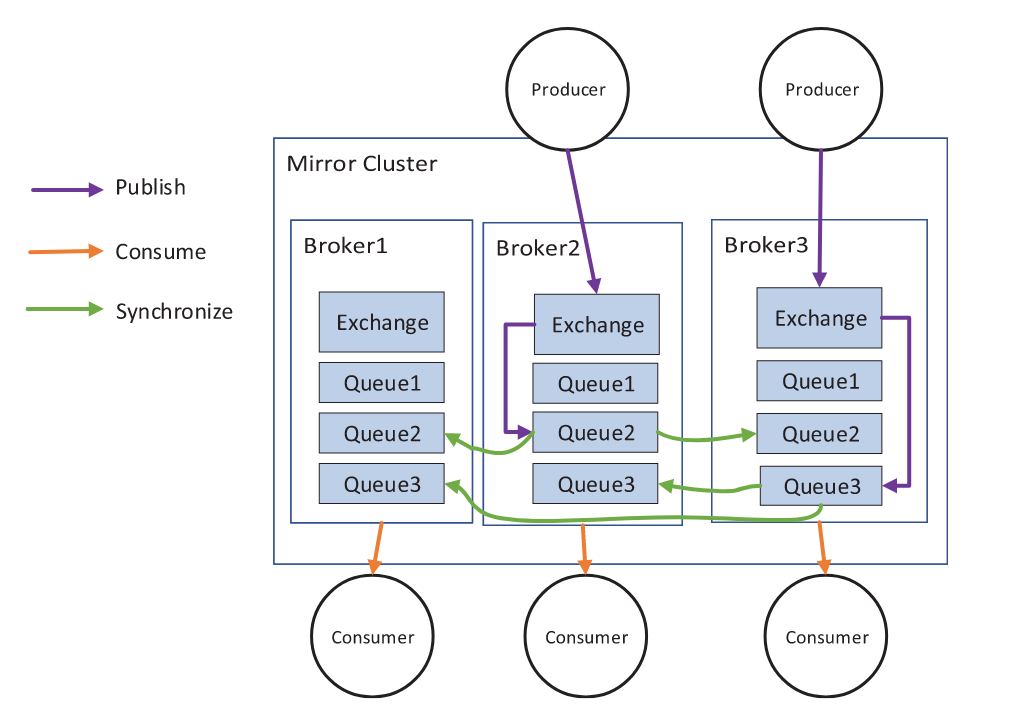
\includegraphics[width=0.9\textwidth]{content/img/Research/Message_Services/rabbitMQArchfairComparisonMessagingSystems.png}
    \caption{Die Architektur des RabbitMQ Systems \cite{fuFairComparisonMessage2021}}
    \label{fig:rabbitMQArchfairComparisonMessagingSystems}
\end{figure}
\FloatBarrier

Das RabbitMQ System ist ein general-purpose Message Broker, da es sehr viele Funktionalitäten implementiert, darunter befinden sich: \cite{toshevLearningRabbitMQBuild2016}

\begin{itemize}
	\item \textbf{Push / Pull Consumption Mode} - RabbitMQ unterstützt sowohl den Push- als auch den Pull-Konsummodus, damit kann das Messaging System perfekt an den Anwendungsfall angepasst werden.
	\item \textbf{Unterstützung von standardisierte Protokolle} - RabbitMQ unterstützt eine Vielzahl von standardisierten Protokollen, darunter AMQP (Advanced Message Queuing Protocol), MQTT (Message Queuing Telemetry Transport), STOMP (Streaming Text Oriented Messaging Protocol) und weitere. Diese Protokolle ermöglichen die Interoperabilität mit verschiedenen Clients und Systemen, was die Integration in bestehende Systeme erleichtert und die Flexibilität erhöht.
	\item \textbf{Point-to-Point und Publish-Subscribe Messaging Models} - RabbitMQ ermöglicht die Kommunikation mit dem Point-to-Point Modell oder mit dem Publish-Subscribe-Modell
	\item \textbf{Disk Nodes oder Memory Nodes für RabbitMQ Cluster} - RabbitMQ bietet die Möglichkeit, Knoten im Cluster als Disk- oder Memory-Knoten zu konfigurieren. Disk-Knoten speichern Nachrichten dauerhaft auf der Festplatte, während Memory-Knoten Nachrichten nur im Arbeitsspeicher speichern.
	\item \textbf{At-Least-Once oder At-Most-Once Zustellungsgarantien} - Durch diese Zustellungsgarantien ist die Kommunikation über RabbitMQ zuverlässig, jedoch ist die Exactly-Once Garantie von RabbitMQ nicht unterstützt. 
\end{itemize}

RabbitMQ bietet eine beeindruckende Bandbreite an Funktionalitäten, die seine Vielseitigkeit und Flexibilität unterstreichen. Diese Merkmale machen es zu einer attraktiven Option für die Integration in bestehende Systeme, da es sich nahtlos in unterschiedliche Architekturen einfügen kann. Trotz dieser Stärken steht RabbitMQ jedoch im Vergleich zu Apache Kafka in Bezug auf Skalierbarkeit und Performance zurück. Insbesondere hinsichtlich des Datendurchsatzes kann RabbitMQ nicht mit der Leistungsfähigkeit von Apache Kafka mithalten. Ein weiterer Unterschied besteht darin, dass RabbitMQ nicht die Möglichkeit bietet, Exactly-Once Semantik zu erreichen, was für bestimmte Anwendungsfälle von entscheidender Bedeutung sein kann.
\cite{toshevLearningRabbitMQBuild2016,fuFairComparisonMessage2021}


